\documentclass[11pts]{report}

\usepackage{qtree}
\usepackage{listings}
\usepackage{amsmath,mathtools}
\usepackage[ruled,longend]{algorithm2e}
\usepackage{tikz}
\usepackage{listings}
\usepackage{graphicx}
\usepackage{xcolor}
\usepackage{array}
\lstset{
    frame=tb, % draw a frame at the top and bottom of the code block
    tabsize=4, % tab space width
    showstringspaces=false, % don't mark spaces in strings
    commentstyle=\color{green}, % comment color
    keywordstyle=\color{blue}, % keyword color
    stringstyle=\color{red} % string color
}

\title{CS 677 Homework \\ Assignment 08}
\author{\textbf{Hai Nguyen}}

\setlength{\topmargin}{-1cm}
\setlength{\oddsidemargin}{0in}
\setlength{\textwidth}{6.5in}
\setlength{\textheight}{8.3in}

\DeclareMathOperator{\Div}{div}
\newcommand{\vect}[1]{\mathbf{#1}}




%%Currently default settings for indentation and symbols.
%%Try these by uncommenting this block!!!
%%Redefine the first level symbols
%\renewcommand{\theenumi}{\fnsymbol{enumi}-}
%\renewcommand{\labelenumi}{\theenumi}
%
%%Redefine the second level symbols
%\renewcommand{\theenumii}{\alph{enumii})}
%\renewcommand{\labelenumii}{\theenumii}
%
%%Redefine the third level symbols
%\renewcommand{\theenumiii}{\roman{enumiii}.}
%\renewcommand{\labelenumiii}{\theenumiii}
%
%%Options for redefining levels


%\arabic
%\alph 
%\Alph
%\roman
%\Roman
%\fnsymbol
%This ^^^ is all you need to change!!

\begin{document}

\maketitle

\begin{enumerate}

% Question 1
\item 

\begin{enumerate} 
\item Kruskal's Algorithm: Order that edges are added to the MST:

\begin{itemize}
\item Add (G, H): [G, H], [A], [B], [C], [D], [E], [F], [I]
\item Add (A, C): [A, C], [G, H], [B], [D], [E], [F], [I]
\item Add (I, H): [A, C], [G, I, H], [B], [D], [E], [F]
\item Add (A, B): [A, B, C], [G, I, H], [D], [E], [F] 
\item Add (C, D): [A, B, C, D], [G, I, H], [E], [F]
\item Add (C, G): [A, B, C, D, G, I, H], [E], [F]
\item Ignore (B, D): [A, B, C, D, G, I, H], [E], [F]
\item Ignore (D, I): [A, B, C, D, G, I, H], [E], [F]
\item Add (G, F): [A, B, C, D, G, I, H, F], [E]
\item Add (C, E): [A, B, C, D, G, I, H, F, E]

\begin{figure}[htbp]
\begin{center}
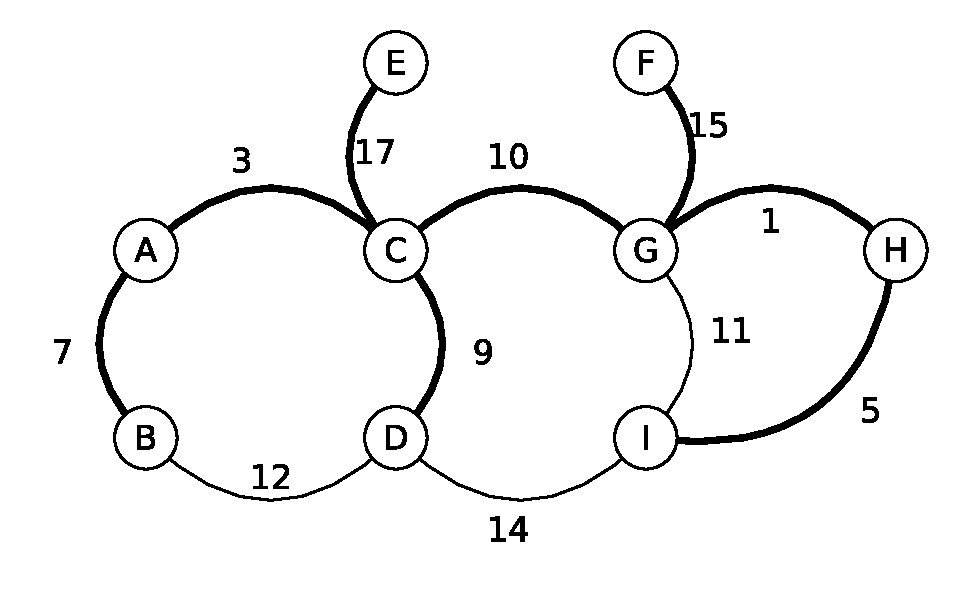
\includegraphics[scale=0.5]{1.pdf}
\caption{Minimum Spanning Tree.}
\label{Fig:1}
\end{center}
\end{figure}

\end{itemize}

\item Prim's Algorithm: Order that edges are added to the MST, starting from vertex A:

\begin{itemize}
\item (A, C) $\to$ (A, B) $\to$ (C, D) $\to$ (C, G) $\to$ (G, H) $\to$ (H, I) $\to$ (G, F) $\to$ (C, E)
\end{itemize}

\end{enumerate}
Both algorithms yield the same MST as shown in Fig. \ref{Fig:1}.

\item Page 602, \textbf{22.2-9}
\begin{itemize}
\item Apply DFS on the given undirected graph. We know that DFS takes $O(V + E)$ to finish. Also, we know that a DFS forms a depth-first forest which will cover all edges and forms a path along the way. This path will also  traverse each edge in $E$ exactly once in each direction because DFS only back-track when it needs to.

\item To find a way out of a maze if we are given a large supply of pennies, we can perform a DFS and use pennies for marking the path that we already traversed through. Each time we traverse through a path we put a penny down and when we back track we put another down. We never traverse in a path with 2 pennies. By this way, we can discover the whole maze and find the way out.
\end{itemize}



\item Page 621, \textbf{22.5-6}
The algorithm works as follows:
\begin{itemize}


   \item Apply \textit{STRONGLY-CONNECTED-COMPONENTS} algorithm to find all strongly connected components in G and component graph $G^{SCC} = (V^{SCC}, E^{SCC})$ : Time $O(V+E)$.
   \item In each strongly connected component, there will be a directed cycle connected all vertices. Start with $E' = \emptyset$. Time: $O(1)$. For each $\text{SCC}$ of $G$, let the vertices in the $\text{SCC}$ be $v_1, v_2, \ldots, v_k$, and add to $E'$ the directed edges $(v_1, v_2), (v_2, v_3), \ldots, (v_{k - 1}, v_k), (v_k, v_1)$. These edges form a simple, directed cycle that includes all vertices of the $\text{SCC}$. Time for all $\text{SCC}$'s: $O(V)$.
  \item   For each edge $(u, v)$ in the graph $G^{\text{SCC}}$, select any vertex $x$ in $u$'s $\text{SCC}$ and any vertex $y$ in $v$'s $\text{SCC}$, and add the directed edge $(x, y)$ to $E'$. Time: $O(E)$.
\item Total time $O(V + E)$.
\end{itemize}


\item Page 663, \textbf{24.3-2}

Given an example of a directed graph with negative-weight edges for which Dijkstra's algorithm produces incorrect answers.

Assume that we apply Dijktra's algorithm to the graph with nagative-weight edges as shown in Figure \ref{Fig:4}. After the aglorithm terminates, we see that the shortest path from the vertice A (the source) to vertice B is 2. However, if we follow the path A $\to$ B $\to$ C $\to$ A $\to$ B, the cost is smaller: 2 + 3 - 6 + 2 = 1 $<$ 2.

\begin{figure}[htbp]
\begin{center}
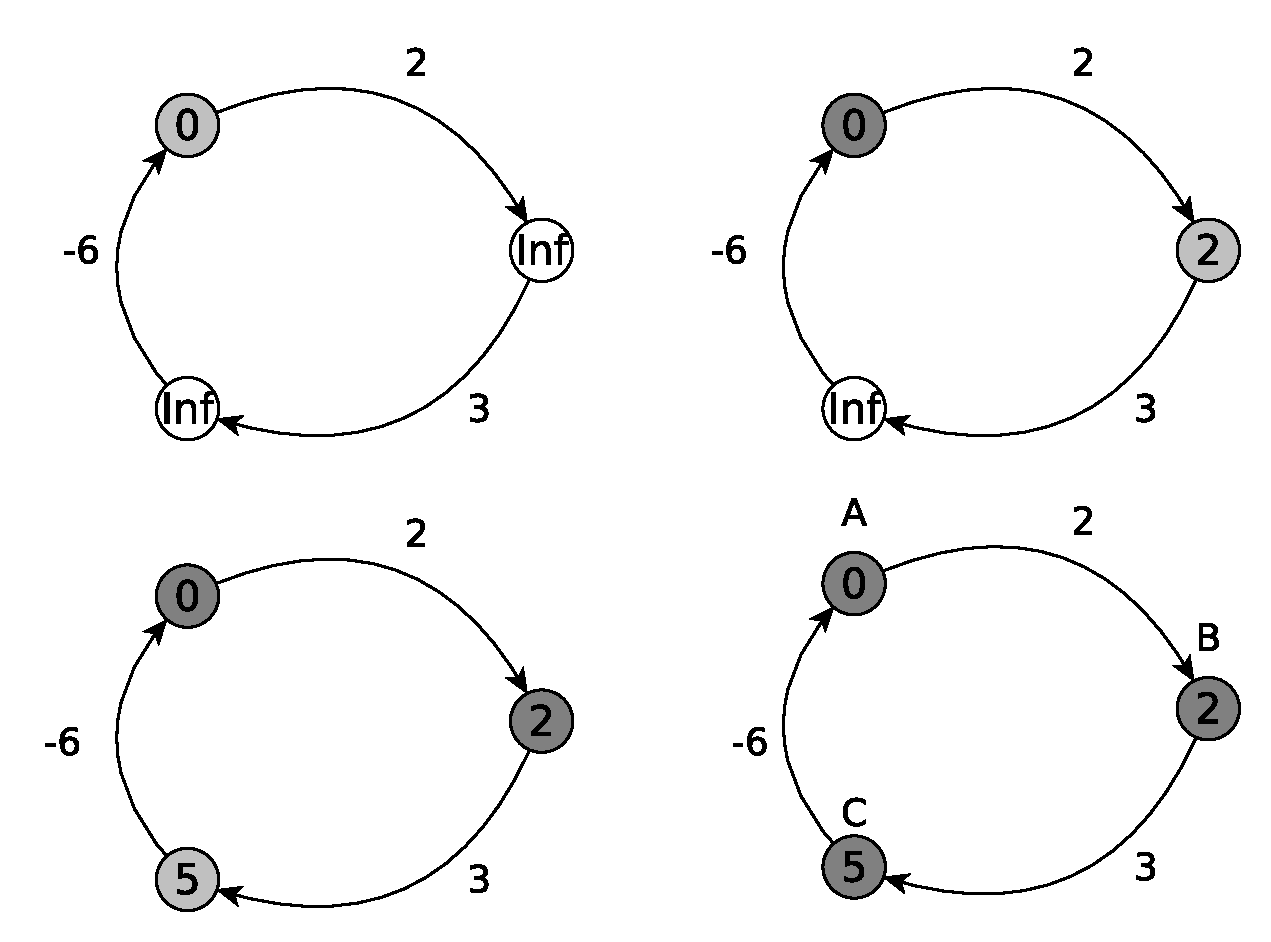
\includegraphics[scale=0.5]{4.pdf}
\caption{Dijkstra's algorithm on negative-weight edges.}
\label{Fig:4}
\end{center}
\end{figure}

The proof of Theorem 24.6 fails at (24.2), because it needs to assusme non-negative weight on path $p2$ (Figure \ref{Fig:5}) in order to have:

\begin{equation*}
y.d = \delta(s,y) \leq \delta(s,u) \leq u.d
\end{equation*}

\begin{figure}[htbp]
\begin{center}
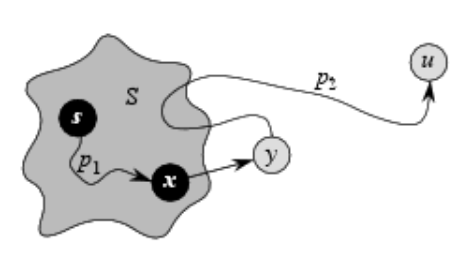
\includegraphics[scale=0.5]{4.png}
\caption{The proof of Theorem 24.6.}
\label{Fig:5}
\end{center}
\end{figure}

\item Page 692, \textbf{25.1-6}
\par Suppose that we are given the completed matrix $L(n,n)$ and the weight matrix $W$, we want to compute the predecessor matrix $\prod$:
\par \textit{Algorithm:}
\par COMPUTE-PI(L, W)
\par \textbf{for} $i = 1:n$
\par \quad \textbf{for} $j = 1:n$
\par \qquad \textbf{for} $k = 1:n$
\par \qquad \quad \textbf{if} $L(i, j) = L(i, k) + W(k, j)$
\par \qquad \qquad $\prod$(i, j) = k
\par The given algorithm run in $O(n^3)$ and for a pair of vertices $(i,j)$, it searches all vertices $k$ in between to see if vertice $k$ is in the shortest-path weights from vertice $i$ to vertice $j$.
\item Page 663, \textbf{24.3-6}
We build a direct graph G' = (V, E) such that each edge $(u, v) \in E$ the associate weight is $W(u,v) = -\text{log}(r(u,v))$, as shown in Figure \ref{Fig:6}. As $0 \leq r(u,v) \leq 1$, we have $W(u,v) \geq 0$. By using Dijkstra's algorithm, we can find the path between the two given vertices such that the total weight is smallest.

\begin{figure}[htbp]
\begin{center}
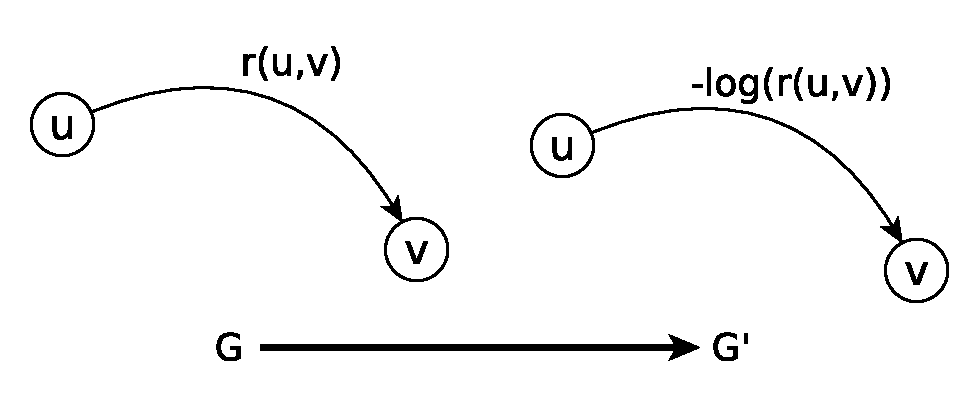
\includegraphics[scale=0.5]{6.pdf}
\caption{Turning G to G'.}
\label{Fig:6}
\end{center}
\end{figure}

We have:
\begin{equation*}
S = \sum_{i=1}^k W_i = -\text{log}(\prod_{i=1}^k r_i)
\end{equation*}
$S$ is minimum so we have $\prod_{i=1}^k r_i$ is maximum, meaning that path is also the most reliable path.
\end{enumerate}

\end{document}
